\section{Eclipse Refactoring Model}

This project involves developing a refactoring plug-in for Eclipse, which work
in the following way:

\begin{figure}
    \centering
    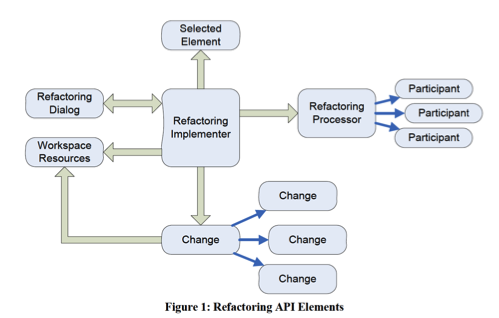
\includegraphics{refactoring_api}
    \caption{Refactoring API Elements}
\label{fig:refact_api}
\end{figure}

\begin{figure}
    \centering
    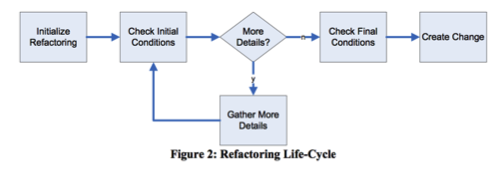
\includegraphics{lifecycle}
    \caption{Refactoring Life-Cycle}
\label{fig:lifecycle}
\end{figure}

\begin{itemize}   

 \item The API for refactoring provides a process-level abstraction upon which
     specific refactorings may be built. 

 \item Figure~\ref{fig:refact_api} shows elements of this abstraction at a
     high level. Arrows between elements represent dependencies.

 \item Once a refactoring has been initiated, an implementer of that
     refactoring is used to coordinate condition checking, gathering details
     about the refactoring, and ultimately produce a series of changes that
     may be applied to the Eclipse workspace to accomplish the refactoring. 

 \item This implementer can extend the abstract class\\
     \lstinline{org.eclipse.ltk.core.refactoring.Refactoring}. The life-cycle
     for this class is shown in Figure~\ref{fig:lifecycle}. 

     % TODO Citation for this stuff?

\end{itemize}
